\documentclass{article}
\usepackage{graphicx}
\usepackage[margin=1.5cm]{geometry}
\usepackage{amsmath}

\begin{document}

\title{Tuesday Reading Assessment: Unit 4, Field Induction and Inductance}
\author{Prof. Jordan C. Hanson}

\maketitle

\section{Memory Bank}

\begin{itemize}
\item $\epsilon = -N \Delta \phi_m /\Delta t$ ... Faraday's Law
\item $\frac{\epsilon_2}{\epsilon_1} = \frac{N_2}{N_1}$ ... Transformer equation.
\end{itemize}

\section{Transformers}

\begin{enumerate}
\item Consider Fig. \ref{fig:trans}, which depicts a \textit{transformer.}  There are two solenoids, the \textit{primary} and \textit{secondary} solenoid.  Using Faraday's law, convince yourself that
\begin{equation}
\frac{V_p}{V_s} = \frac{N_P}{N_S}
\end{equation}
This is because the flux is the same through each solenoid. \\ \vspace{1cm}
\item A battery charger meant for a series connection of ten nickel-cadmium batteries (total emf of 12.5 V DC) needs to have a 15.0 V output to charge the batteries. It uses a step-down transformer with a 200-loop primary and a 120 V input. (a) How many loops should there be in the secondary coil? (b) If the charging current is 16.0 A, what is the input current? \\ \vspace{1cm}
\end{enumerate}

\begin{figure}[hb]
\centering
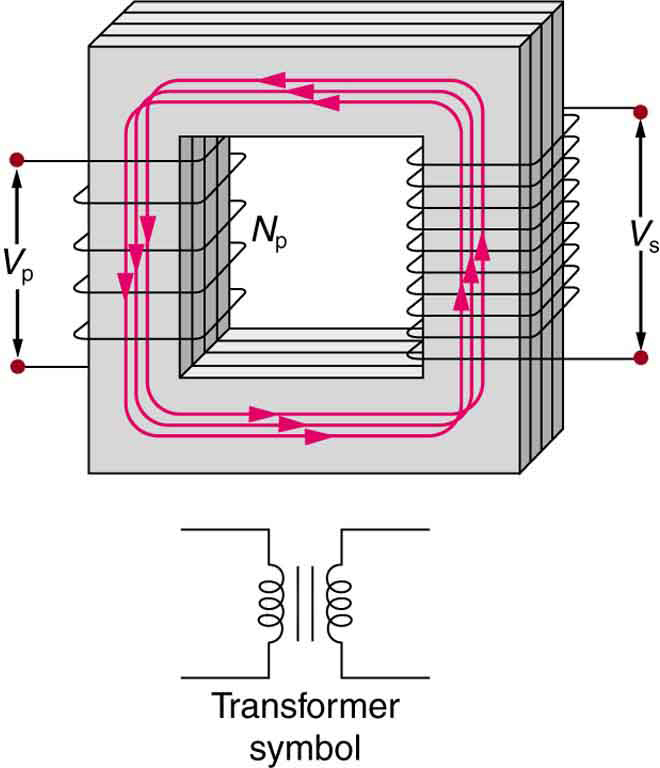
\includegraphics[width=0.3\textwidth]{transformer.jpeg}
\caption{\label{fig:trans} A basic diagram of a transformer with primary and secondary coils.  The iron core magnetizes and transfers flux from one coil to the other.}
\end{figure}
\end{document}
